% Chapter Template

\chapter{Methodology} % Main chapter title

\label{Chapter4} % Change X to a consecutive number; for referencing this chapter elsewhere, use \ref{ChapterX}

\lhead{Chapter 4. \emph{Methodology}} % Change X to a consecutive number; this is for the header on each page - perhaps a shortened title

%----------------------------------------------------------------------------------------
%	SECTION 1
%----------------------------------------------------------------------------------------

\section{Many Body Methods}

As previously discussed in Chapter \ref{Chapter1}, the aim of many body quantum mechanics is to find either the exact, or a reasonable approximation to the many body systems wave function $\Psi$. This wave function resides in Fock space, a space spanned by all possible Slater Determinants constructed by the single-particle states from the corresponding one-body problem. This wave function may be written (for $N$ particles)

\begin{equation}
\vert \Psi \rangle = c_0 \vert \Phi_0 \rangle + \sum_{ai} c_{ai }\vert \Phi_i^a \rangle +  \sum_{abij} c_{abij} \vert \Phi_{ij}^{ab} \rangle + ... + \sum_{ab...N_a ij...N_i} c_{ab...N_a ij...N_i} \vert \Phi_{ij...N_i}^{ab...N_a} \rangle.
\label{eqn:fullCI}
\end{equation}

To determine the full wave function we therefore need a complete single-particle basis as well as the means to project it onto Fock space, determining its coefficients. In general, we may consider the process of generating the full wave function from the reference state to be an operator acting on the reference state

\begin{equation}
\vert \Psi \rangle = \hat{\Omega} \vert \Phi_0 \rangle .
\label{eqn:reference_operator}
\end{equation}

\section{The Hartree Fock Method}

A complete basis often means an infinite number of single-particle states, which in turn means an infinite number of Slater determinants. Such a system is not possible to implement computationally, so we may instead seek ways of truncating our basis. As previously discussed in chapter 1 and 2, the precision of our solution will now depend on how much of the exact wave function is present in the retained basis. To this end, we will seek a single-particle basis that ensures that most of the systems wave function is present in one single Slater determinant.

The \emph{Hartree Fock method} is a way of optimizing the single-particle states so that a single Slater determinant gives a decent representation of the system. The resulting Slater determinant may serve as a starting points for several so called \emph{post Hartree Fock methods}, such as MBPT (many body perturbation theory), CI (Configuration Interaction) or CCM (Coupled Cluster Method). \cite{ShavittBartlett2009} For this reason,we will give it some special attention.

The first development of the method is attributed to Douglas Rayner Hartree who in 1927 introduced a procedure he called \emph{the self consistent field method} \cite{Thijssen} but which was later named the \emph{Hartree Fock Rothaan} method. Although it was originally distinguished between this method and what was called the Hartree Fock method, this distinction has now been lost \cite{ShavittBartlett2009}, and the name normally refers to the method that will be discussed in the following sections.

\subsection{The variational principle}

The Hartree Fock method is based on the variational principle, which states that when we evaluate the inner product of the hamiltonian on \emph{any} normalized wave function, the resulting energy will be an upper bound to the ground state energy. \cite{Griffiths2005}

\begin{equation}
E_0 \leq \langle \Psi_{trial} \vert \hat{H} \vert \Psi_{trial} \rangle.
\label{eqn:variational}
\end{equation}

Such wave functions are commonly called \emph{trial} wave functions. 

This principle provides us with an approximate scheme, and by parameterizing the trial wave function we may improve upon this solution.

\subsection{Expanding the single-particle states}

The parametrization of the Slater determinant is performed by letting each single-particle state be represented by a linear combination of the eigenstates to the corresponding one body problem. If we refer to the linear combinations by $\psi$ with Latin indices and the basis states as $\phi$ with Greek indices, we may write this as

\begin{equation}
\vert \psi_i \rangle = \sum_\alpha^A c_{\alpha,i} \vert \phi_{\alpha,i} \rangle .
\label{eqn:expanding_sp_states}
\end{equation}

Note that we truncate the basis at the A'th function to make computations possible. More functions generally means a better representation. 

In accordance with the variational principle, we now want to determine the coefficients $c_{\alpha, i}$ in such a way that we minimize the energy. We should therefore insert the expanded single-particle states into the energy equation (\ref{eqn:many_body_energy}) that we derived in chapter 1, so we find

\begin{multline}
 \epsilon _0 = \sum _{\alpha, \beta}^A C_{\alpha,i}^{*}C_{\beta,i} \sum _{i}^N \langle \phi _i | \hat{f}(\mathbf{x_i}) | \phi _i \rangle + \\ 
 \sum _{\alpha,\beta, \gamma, \delta} ^A C_{\alpha,i}^{*}C_{\beta,j}^{*}C_{\gamma,i}C_{\delta,j} \frac{1}{2}\sum _{i, j\neq i}^N \langle \phi _{\alpha,i}\phi _{\beta,j}| \hat{v}(\mathbf{x_i},\mathbf{x_j}) |\phi _{\gamma,i}\phi _{\delta,j} \rangle.
\label{eqn:greek_HF}
\end{multline}

The way in which we now have set up the system, we may consider the coefficients to be a matrix with $A$  rows (Greek letters) and $N$ columns, where $N$ is the number of particles. In the special case where diagonal elements are one and all others zero, we find the same system as we have discussed up to this point.

\subsection{Ensuring orthonormality}

The trial wave function is now parameterized by the introduction of coefficients. When varying or optimizing these coefficients to minimize the energy, we must be careful to constrain the orthonormality of the states (remember, failing to do so will cause a violation of the Pauli Principle). Mathematically this constraint may be written

\begin{equation}
\langle \psi_i \vert \psi_j \rangle = \sum_{\alpha}^A c_{\alpha, i}^*c_{\alpha, j} = \delta_{ij}.
\label{eqn:orthonormality}
\end{equation}

To this end, we may use \emph{Lagrange's method of undetermined multipliers} \cite[p.116]{Szabo} (or simply  \emph{Lagrange multipliers}), and set up a functional to be minimized with the constraint described above:

\begin{equation}
 F\big( E\big( c \big), \lambda \big) = E\big( c \big) - \sum _i^N \lambda _i \sum _{\alpha}^A c_{\alpha,i}^{*} c_{\alpha,i}.
 \label{lagrange_minim}
\end{equation}

To find a minimum for this functional we must solve

\begin{equation}
\frac{\partial}{\partial c_{\alpha,i}^{*}} F\big( E\big( c \big), \lambda \big) = 0.
\label{eqn:partialset}
\end{equation}

For a step by step solution, the reader is referred to Thijssen's \emph{Computational Physics} \cite{Thijssen} or Szabo's \emph{"Modern Quantum Chemistry"} \cite{Szabo}. In the following we will just state the solution consistent with how it is given in these sources.

\subsection{The Hartree Fock Equations}

By solving \ref{eqn:partialset}, we obtain a set of coupled one particle eigenvalue problems given by

\begin{multline}
\lambda _k C_{\alpha,i} =  
\sum _{\beta}^A\sum _{i}^N C_{\beta,i}\langle \alpha |\hat{f}(\mathbf{x_i}) | \beta \rangle + 
\sum _{\beta,\gamma,\delta}^A \sum _i^N C_{\beta,j}^{*}C_{\gamma,i}C_{\delta,j}\langle \alpha \beta |\hat{v}(\mathbf{x_i},\mathbf{x_j}) .|\gamma \delta \rangle _{AS}
 \label{eqn:HF1}
\end{multline}

These are known as the Hartree Fock equations, and by identifying $\lambda$ as the Hartree Fock energy \cite{hh4480} we may write them as

\begin{equation}
\epsilon_i^{HF} C_{\alpha,i} =  
\sum_{\beta} \Big{(}  {\langle \alpha |\hat{f}(\mathbf{x_i}) | \beta \rangle + \sum_j^N \sum_{\gamma \delta}{C_{j \gamma} C_{j \delta}  \langle \alpha \gamma |\hat{v}(\mathbf{x_i}) | \beta \delta \rangle } } \Big{)},
 \label{eqn:HF2}
\end{equation}

or simply 

\begin{equation}
\sum_\beta f_{\alpha \beta}^{HF} C_{i \beta} = \epsilon_i^{HF} C_{\alpha,i} .
\label{eqn:hartreefock}
\end{equation}

The matrix $ \hat{f}^{HF} $ is commonly known as the \emph{Fock} operator, and has dependence upon all the spin orbitals. \cite{ShavittBartlett2009}. As a consequence, a first guess for the coefficients is likely to be inconsistent when evaluating the left hand side and right hand side of \ref{eqn:hartreefock}, so they are normally solved in an iterative manner. This is why the method was initially named the self consistent field method; the field produced by the particles should be consistent with the field "felt" by each particle.

A set of single particle states that fullfill \ref{eqn:hartreefock} are called the \emph{canonical Hartree Fock wave function}, while the constituent states are called \emph{the canonical spin orbitals}. 

\subsection{Koopman's theorem}

The HF energy for any state $p$ may be compactly written

\begin{equation}
\epsilon^{HF}_p = \langle p \vert \hat{h}_0 \vert p \rangle + \frac{1}{2} \sum_{j} \langle pj \vert  \vert pj \rangle .
\label{eqn:hf_koopman}
\end{equation}

This is the energy associated with each orbital expanded as a linear combination of single-particle states. Each fermion in the system will then have an associated Hartree Fock energy.

Koopman's theorem states that for closed-shell Hartree Fock calculations, the ionization energy of the system is equal to the negative of the outermost hole state in the system. \cite{Thijssen} The ionization energy may then be computed by performing a Hartree Fock procedure, whereby we calculate only the outermost occupied orbital in equation. \ref{eqn:hf_koopman}

\subsection{Restricted and unrestricted Hartree Fock}

There are multiple ways of implementing the Hartree Fock equations. For closed shell systems, such as $He$, $H_2$ and $Be$, the electrons (in general fermions), may be assumed to be paired with opposite spin electrons. In the restricted Hartree Fock method (RHF), we consider only systems where all fermions are paired with opposite spin particles. This lets us scale down the computation, but it will naturally give poor results for systems where no such pairing occurs, for example in the case where two $H$ atoms are interacting over a great distance.

For systems with singly occupied states (unpaired fermions, typically odd numbered) the restriction of spin-pairing is no longer valid.

To take this into account, we set up two Fock matrices; one for each spin orientation. The resulting system is

\begin{equation}
\hat{F}_\alpha(C_\alpha, C_\beta) C_\alpha = \hat{S} C_\alpha \epsilon_\alpha.
\end{equation}

\begin{equation}
\hat{F}_\beta(C_\alpha, C_\beta) C_\beta = \hat{S} C_\beta \epsilon_\beta.
\end{equation}

The ground state energy will be a function of the eigenvectors of these two matrices. The dependency of opposite spin coefficients in the Fock matrices is due to the direct- or coulomb term from the two particle integrals. \cite[p.241]{Szabo} This latter approach is called the \emph{unrestricted Hartree Hock} method.



\section{Post Hartree Fock Methods}

While the HF reference state may account for important correlations such as the Pauli exclusion principle and interactions with the mean field, it will lack the instantaneous coulomb repulsion between the electrons. For this reason, certain correlations may never be fully accounted for with the Hartree Fock method alone. Figure \ref{fig:correlation}  illustrates what is often defined as the correlation energy; the energy attributed to correlations beyond the mean field.

\begin{figure}[p]
    \centering
    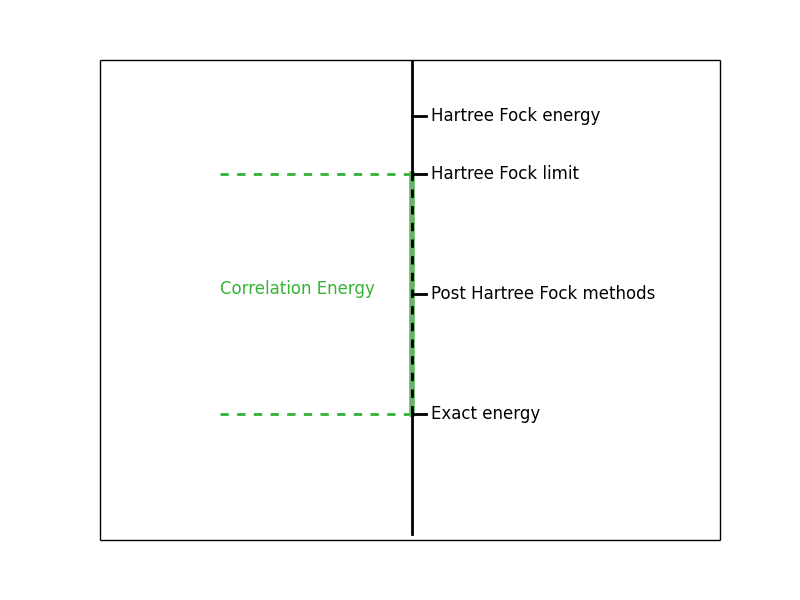
\includegraphics[width=0.8\textwidth]{correlation}
    \caption{Correlations beyond the Hartree Fock energy. At the so called Hartree Fock limit, we have achieved the best possible description of our system using the mean field approach. The energy unaccounted for by the reference state is commonly referred to as the \emph{correlation energy}. The so called \emph{post Hartree Fock} methods, such as the Coupled Cluster method, will help us include even more correlations and bring us closer to the exact energy.}
    \label{fig:correlation}
\end{figure}


A byproduct of the Hartree Fock method is very often particle states above the Fermi level. Such states may be present even before the Hartree Fock method is applied, for example in cases where Gaussian basis sets are used, or they may be derived from the spin treatment in the Restricted Hartree Fock procedure.

These particle states will allow us to create excited Slater determinants for use in the so called \emph{post Hartree Fock} methods. By including excited Slater determinants, such methods may account for the correlations due to the push or pull exerted by the fermions. One such approach is the Coupled Cluster (CC) method, which is a central subject in this thesis. Alongside CC, we have several other methods such as Configuration Interaction (CI) or Many Body Perturbation Theory (MBPT). 

Important insight into various physical systems may be gained by comparing results amongst these methods, as they all have their strengths and weaknesses. Prior to the treatment of the CC method in chapter 5, we shall therefor just briefly discuss some of these alternative post Hartree Fock methods, so a meaningful comparison of results may be performed in the final chapter of this thesis.

\subsection{Configuration Interaction}

The Configuration Interaction (CI) method, sometimes referred to as the \emph{method of superposition of configurations} \cite{Harris} is based on the expansion of the systems wave function into a linear combination consisting of the reference Slater determinant and a (possibly infinite) set of excited versions of this Slater determinant, as briefly noted in the introduction to this chapter.

\begin{equation}
\vert \Psi \rangle = c_0 \vert \Phi_0 \rangle + \sum_{ai} c^{a}_i\ vert \Phi_i^a \rangle +  \sum_{abij} c^{ab}_{ij} \vert \Phi_{ij}^{ab} \rangle + ... + \sum_{ab...N_a ij...N_i} c^{ab...N_a}_{ij...N_i} \vert \Phi_{ij...N_i}^{ab...N_a} \rangle.
\label{eqn:fullCI}
\end{equation}

The CI method is considered to be the mathematically simplest technique for inclusion of correlations beyond the mean field. \cite{Harris} The operator that brings us from the reference Slater determinant to the true system wave function may be written

\begin{equation}
\vert \Psi \rangle = \Omega \vert  \Phi_0 \rangle = (c_0 + \hat{C}) \vert  \Phi_0 \rangle,
\end{equation}

where

\begin{equation}
\hat{C} = \sum_{ai} c^{a}_i \Cr{a} \An{i}+  \sum_{abij} c^{ab}_{ij} \Cr{a} \Cr{b} \An{j} \An{i} + ... + \sum_{ab...N_a ij...N_i} c^{ab...N_a}_{ij...N_i} \Cr{a} \Cr{b} ... \Cr{N_a} \An{N_i} ... \An{j} \An{i}.
\end{equation}

The coefficients $c$ are then obtained by variational means, by minimizing 

\begin{equation}
E = \langle \Psi \vert \hat{H} \vert \Psi \rangle.
\label{eqn:fullCIvar}
\end{equation}

We shall not go into more details concerning this. The reader is referred to for example \cite[p.177]{Harris} for a more complete treatment. 

We will however make some general observations concerning the CI method. 

\subsection{Full Configuration Interaction}

The equation \ref{eqn:fullCIvar} is solvable, but at great computational cost. The number of excited Slater determinants, and thereby the number of coefficients, scales \emph{factorially} with the number of particle- and hole states.

The practical consequence is that inclusion of all Slater determinants is only possible for smaller systems unless some truncation of the Slater determinants is introduced. From a physical point of view, we may have systems where no single excitation is allowed, and for this reason the singly excited coefficients may be excluded with no loss of precision.

The various truncations are commonly referred to as CIS for inclusion of single excitations, CISD for single and double 
excitations and so on. 

\subsection{Configuration Interaction Quantum Monte Carlo}

We will later in this thesis compare results with results from a so-called FCIQMC (Full Configuration Quantum Monte Carlo) calculation. This approach determines the FCI coefficients by stochastic processes. \cite{Booth2013} \cite{Leikanger2013} Such results are valuable for our purpose, since they basically provide us with the exact ground state energy for smaller system, which will allow us to evaluate to which degree the method accounts for correlations in the system.

\subsection{Many Body Perturbation Theory}

As opposed to the Hartree Fock method, Configuration Interaction and Coupled Cluster methods, \emph{Many Body Perturbation Theory} (MBPT) offers a none iterative approach to approximating the systems wave function. The following derivation is based on the one in \cite{ShavittBartlett2009} and \cite{hh4480}.

The basic idea is to arrange the hamiltonian into two parts

\begin{equation}
\hat{H} = \hat{H}_0 + \hat{V}.
\end{equation}

This is very similar to what we have done so far, as we seek an $\hat{H}_0$ which is exactly solvable (which yields the single-particle basis) and a $\hat{V}$ that will be treated as a perturbation. The solution to the unperturbed problem is given

\begin{equation}
\hat{H}_0 \vert \Phi_0 \rangle = W_0 \vert \Phi_0 \rangle.
\end{equation}

As for Configuration Interaction, we have the exact ground state wave function for our system represented by a linear combination of Slater determinants, where we assume the first term (reference state) to be the dominating term

\begin{equation}
\vert \Psi_0 \rangle = \vert \Phi_0 \rangle + \sum_m^\infty c_m \vert \Phi_m \rangle.
\end{equation}
 
We then assume an intermediate normalization $\langle \Phi_0 \vert \Psi_0 \rangle = 1$ and project our Schödinger equation onto $\langle \Phi_0 \vert$ so we have

\begin{equation}
\langle \Phi_0 \vert \hat{H} \vert \Psi_0 \rangle = \langle \Phi_0 \vert \hat{H}_0 + \hat{V} \vert \Psi_0 \rangle = E.
\end{equation}

We still doesn't really know what the ground state energy is, but we may subtract the \emph{unperturbed} energy to find and expression for the correlation energy

\begin{equation}
\langle \Phi_0 \vert \hat{V} \vert \Psi_0 \rangle = E - W_0 = \Delta E.
\end{equation}

We may add and subtract a term $\omega \vert \Psi_0 \rangle$ to the expression above and regroup it to find

\begin{equation}
\vert \Psi_0  \rangle = \frac{1}{(\omega - \hat{H}_0)} (\hat{V} + \omega - E) \vert \Psi_0 \rangle .
\label{eqn:pt_1}
\end{equation}

By interpreting the term $\omega$ in different ways, we will arrive at the various Many Body Perturbation schemes.

The system's true wave function is still unknown, but it is fully possible to expand it in a known basis $\{\phi_n \}$, so that

\begin{equation}
\vert \Psi \rangle = (\hat{P} + \hat{Q})\vert \phi_0 \rangle,
\end{equation}

where we have the projection operator $\hat{P} = \vert \phi_0 \rangle \langle \phi_0 \vert$, $\hat{P} = \hat{P}^\dagger = \hat{P}\hat{P}$ and $\hat{Q} = \sum_{m} \vert \phi_m \rangle \langle \phi_m \vert$. \cite{ShavittBartlett2009} We insert this into Eq. (\ref{eqn:pt_1}) to find

\begin{equation}
\vert \Psi_0  \rangle = \phi_0 \rangle + \sum_i^\infty \Big{(} \frac{1}{(\omega - \hat{H}_0)} (\hat{V} + \omega - E) \Big{)}^i \vert \phi_0 \rangle ,
\label{eqn:pt_2}
\end{equation}

so that the correlation energy takes the form

\begin{equation}
\Delta e = \sum_i^\infty  \hat{V} \Big{(} \frac{1}{(\omega - \hat{H}_0)} (\hat{V} + \omega - E) \Big{)}^i \vert \phi_0 \rangle .
\label{eqn:pt_2}
\end{equation}

By letting $\omega = E$, we obtain the so called Brillouin-Wigner Perturbation Theory, or we may let $\omega = W_0$ to obtain Rayleigh-Schrödinger Perturbation Theory (RSPT). In the Brillouin-Wigner case, a possible solution would involve iterations and self consistence as in Hartree Fock, CI and CC, while in the RSPT case we end up with terms that corresponds to different orders of the correlation energy, so we have

\begin{equation}
\Delta e = \Delta E^{(1)}+\Delta E^{(2)}+\Delta E^{(3)}+... ,
\end{equation}

Where

\begin{equation}
\Delta E^{1} = \langle \phi_0 \vert \hat{V} \vert \phi_0 \rangle,
\end{equation}

\begin{equation}
\Delta E^{2} = \langle \phi_0 \vert \hat{V}  \frac{\hat{Q}}{(W_0 - \hat{H}_0)}  (\hat{V} - \Delta E) \vert \phi_0 \rangle,
\end{equation}

\begin{equation}
\Delta E^{3} = \langle \phi_0 \vert \hat{V} \frac{\hat{Q}}{(W_0 - \hat{H}_0)}  (\hat{V} - \Delta E) \frac{\hat{Q}}{(W_0 - \hat{H}_0)}  (\hat{V} - \Delta E)  \vert \phi_0 \rangle,
\end{equation}

..and so on.






\subsection{The linked diagram theorem}

We will not go into any further detail on the Many Body Perturbation Methods methods, but we should note an important theorem introduced by Goldstone \cite{Goldstone1957} \cite[p.152]{ShavittBartlett2009}. 

Computations of the different orders in Rayleigh-Schrödinger Perturbation Theory may be performed diagrammatically. Based on a set of rules (see for example \cite{ShavittBartlett2009}), we may generate a lot of diagrams corresponding to the possible contractions operators present in each order of the perturbation. Actually, the diagrammatic rules will produce a lot more diagrams then what is actually needed in order to calculate the correlation energy. 

The \emph{linked diagram theorem} is a simple way of getting rid of a lot of these excess diagrams.

A diagram may be called \emph{linked} if all parts of the diagram is linked with each other by contractions. Unlinked diagrams will be easily identified as it is possible to split them into smaller parts by drawing lines through them without crossing any lines in the diagram. 

The linked diagram theorem states that these diagrams do not contribute to the correlation energy or the wave function. 

In the equations (\ref{eqn:pt_2}) for Rayleigh-Schrödinger Perturbation Theory, we will therefore only have to consider terms where contractions occur between all operators in each term (ASK MORTEN). 

\section{Other many body methods}

Some notable alternatives to the Hartree Fock and post Hartree Foc approaches are Quantum Monte Carlo (QMC) and density functional theory (DFT). 



Use Thijssen here (Quantum Monte Carlo, DFT, 



